\documentclass[10pt,xcolor=table]{beamer}

\usetheme[subsectionpage=progressbar]{metropolis}
\setbeamertemplate{itemize subitem}{--}
\setbeamerfont{caption}{size=\footnotesize}
\usepackage{appendixnumberbeamer}

\usepackage{listings}
\lstset{
  basicstyle=\footnotesize\ttfamily,
  backgroundcolor = \color{gray!20}
}
\lstdefinestyle{c}{language=C,
  keywordstyle=\bfseries\color{green!40!black},
  commentstyle=\itshape\color{purple!40!black},
  % identifierstyle=\color{blue},
  stringstyle=\color{orange}
}
\lstdefinestyle{shell}{language=sh,
  commentstyle=\itshape\color{purple!40!black},
  moredelim=**[is][\only<2->{\color{red}}]{@}{@},
  moredelim=**[is][\only<3>{\color{blue}}]{¿}{¿}
}
\lstdefinestyle{asm}{language=[x86masm]Assembler,
  commentstyle=\itshape\color{purple!40!black},
}
\lstdefinestyle{valgrind}{basicstyle=\footnotesize\ttfamily,
  backgroundcolor = {},
}
\usepackage{caption}
\captionsetup[lstlisting]{font={small,tt}, labelformat=empty,
  labelsep=none}

\usepackage{booktabs}
\usepackage[scale=2]{ccicons}

\usepackage{pgfplots}
\usepgfplotslibrary{dateplot}

\usepackage{expl3}
\ExplSyntaxOn
\int_zero_new:N \g__prg_map_int
\ExplSyntaxOff
\usepackage{tikz}
\usetikzlibrary{tikzmark,decorations.pathreplacing,calligraphy}

% Figure's path
\graphicspath{{./figs/}}

\title{Optimization and Profiling of HPC Applications}
\subtitle{using free software resources}
\date{\today}
\author{Emilio J. Padrón González}
 \institute{\href{mailto:emilioj@udc.gal}{\nolinkurl{emilioj@udc.gal}}
   -- \url{http://gac.udc.es/~emilioj}\\Computer Architecture Group
   -- Universidade da Coruña}

\begin{document}

\maketitle

\begin{frame}{Outline}

  \setbeamertemplate{section in toc}[sections numbered]
  \tableofcontents[hideallsubsections]

\end{frame}

\begin{frame}{Contents: Lesson 1 and 2}

  \setbeamertemplate{section in toc}[sections numbered]
  \setbeamertemplate{subsection in toc}[ball unnumbered]
  \tableofcontents[sections={1-2}]

\end{frame}



\section{Introduction}

\subsection{Free Software}

\frame{
  \frametitle{What we means by: [\ldots] using \underline{Free
      Software} resources}

  \begin{tikzpicture}[remember picture,overlay]
    \node[xshift=-2cm,yshift=-2.5cm] at (current page.north east) {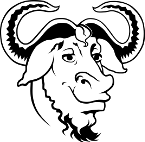
\includegraphics[width=2cm]{gnu.png}};
  \end{tikzpicture}

  \vfill

  \begin{quote}
    Free as in Freedom~\footnote{\ldots not as in \emph{free beer}: \url{http://www.oreilly.com/openbook/freedom}}
  \end{quote}

  \vfill

  \begin{itemize}
  \item Free software definition according to FSF:
    \url{http://www.gnu.org/philosophy/free-sw.html}
  \item Similar terms: \emph{Open Source}, \emph{FLOSS} (Free/Libre
    and Open Source Software)
  \end{itemize}
}

\subsection{HPC \& Computer Organization and Architecture basics}

\frame{
  \frametitle{Forms of parallel computing}

  \begin{itemize}
  \item Bit-level parallelism
  \item Instruction-level parallelism (ILP)
  \item Data-level parallelism (DLP)
  \item Task-level parallelism (TLP)
  \end{itemize}
}

\frame{
  \frametitle{A taxonomy of computer architectures}

  Flynn's taxonomy (1966!)

  \begin{description}
  \item[SISD] Single Instruction stream; Single Data stream
  \item[MISD] Multiple Instruction stream; Single Data stream
  \item[SIMD] Single Instruction stream; Multiple Data stream
    \only<2->{
      \begin{description}
      \item[\alert{\footnotesize (variant)} SIMT] Single Instruction; Multiple Threads
      \end{description}
    }
  \item[MIMD] Multiple Instruction stream; Multiple Data stream
    \only<3>{
      \begin{description}
      \item[\alert{\footnotesize (typically)} SPMD] Single Program; Multiple Data
      \end{description}
    }
  \end{description}

  \begin{figure}
    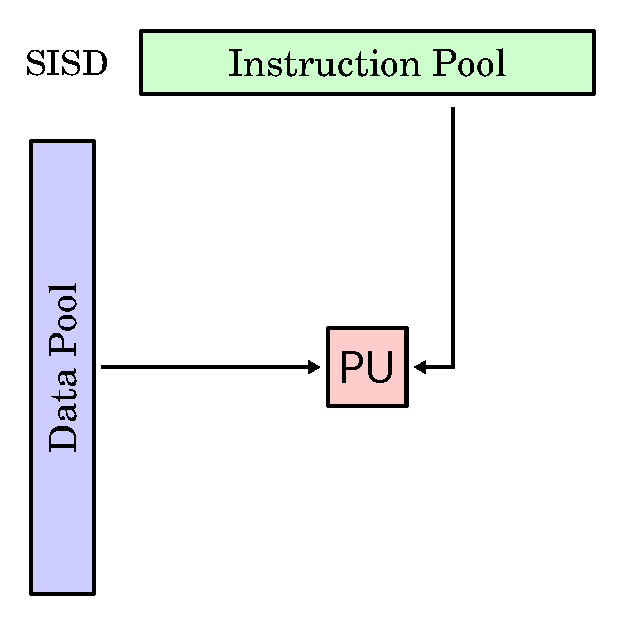
\includegraphics[width=0.25\textwidth]{SISD}~
    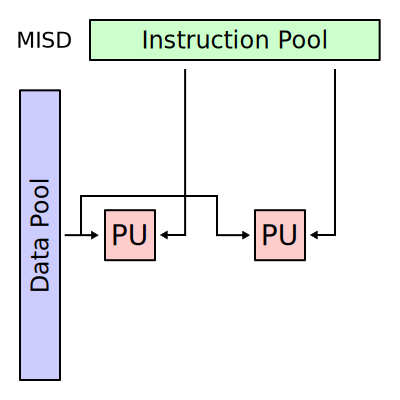
\includegraphics[width=0.25\textwidth]{MISD}~
    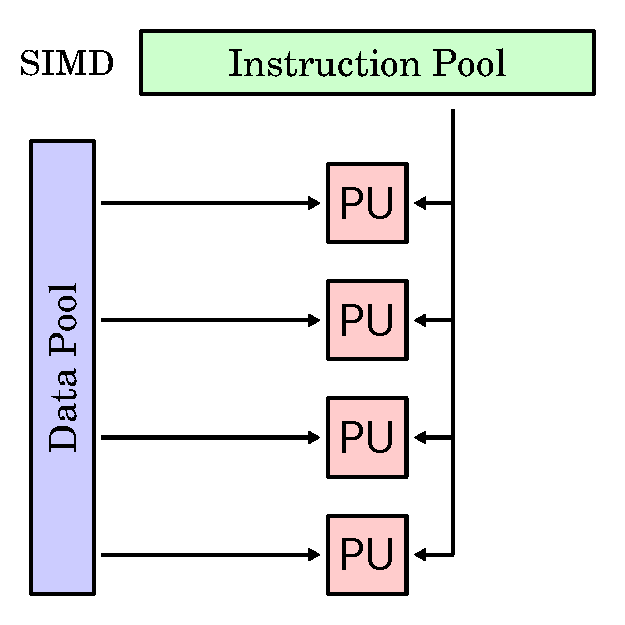
\includegraphics[width=0.25\textwidth]{SIMD}~
    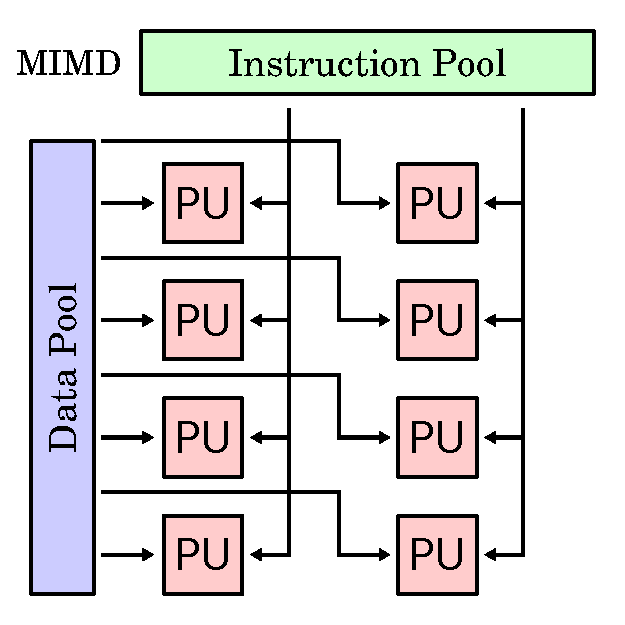
\includegraphics[width=0.25\textwidth]{MIMD}
    \caption{By I, Cburnett, CC BY-SA 3.0,
      \url{https://commons.wikimedia.org/w/index.php?curid=2233537}}
  \end{figure}
}

\frame{
  \frametitle{Parallel processing in Flynn's taxonomy}

  \begin{block}{SISD: exploit ILP}
    \begin{itemize}
    \item Superscalar processors
    \item Pipelining
    \end{itemize}
  \end{block}

  \begin{block}{SIMD: exploit data parallelism}
    \begin{itemize}
    \item Array and Vector processors
    \item Vector extensions in general purpose CPU
    \item GPGPU or similar approaches based on co-processors
    \end{itemize}
  \end{block}

  \begin{block}{MIMD: exploit task parallelism}
    \begin{itemize}
    \item Multicore, multiprocessor and multicomputer architectures
    \end{itemize}
  \end{block}

}

\frame{
  \frametitle{The memory}

  \begin{figure}
    \begin{overprint}
      \onslide<1>
      \includegraphics<1>[width=\textwidth]{memhierarchy}
      \onslide<2>
      \includegraphics<2>[width=\textwidth]{memhierarchy_detail}
    \end{overprint}
    \caption{Memory levels in a computer}
  \end{figure}
}

\frame{
  \frametitle{CPU \& Cache memory levels}

  \begin{figure}
    \begin{columns}
      \column{0.4\textwidth}{
        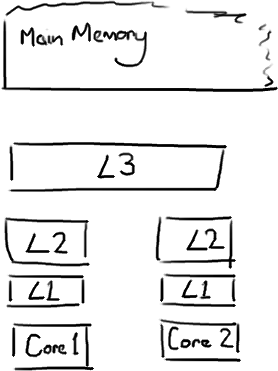
\includegraphics[width=0.5\textheight]{CPUCache}
      }

      \column{0.45\textwidth}{
        \begin{table}\footnotesize
          \caption{Memory latencies from CPU}
          \begin{tabular}{lll}
            \toprule
            \parbox[t]{1.3cm}{\bf Latency\\ CPU to...}
            & \parbox[t]{1.35cm}{\bf CPU cycles\\(approx.)}
            & \parbox[t]{1cm}{\bf Time\\ (approx.)}\\[0.5cm]
            Main mem & & \~{}60-80ns\\
            QPI transit & & \~{}20ns\\
            L3 cache & \~{}40-45 cycles & \~{}15ns\\
            L2 cache & \~{}10 cycles & \~{}3ns\\
            L1 cache & \~{}3-4 cycles & \~{}1ns\\
            Register & 1 cycle\\
            \bottomrule
          \end{tabular}
        \end{table}
      }
    \end{columns}
    \vspace*{-0.4cm}
    \caption{Memory hierarchy in a multi-core CPU~\footnote{2010
        numbers. More up-to-date info:
        \url{http://gist.github.com/eshelman/343a1c46cb3fba142c1afdcdeec17646}}\\
      {\scriptsize By Trisha Gee, CC BY 3.0,
        \url{http://trishagee.github.io/post/dissecting_the_disruptor_why_its_so_fast_part_two__magic_cache_line_padding}}
    }
  \end{figure}
}

\frame{
  \frametitle{Cache and cache lines}

  Cache: exploiting locality
  \begin{itemize}
  \item temporal
  \item spatial
  \end{itemize}

  \pause

  \begin{figure}
    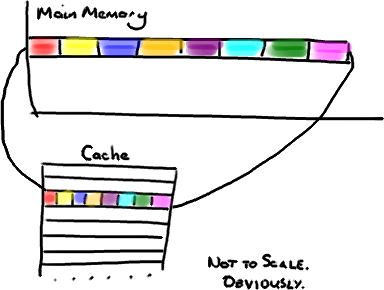
\includegraphics[width=0.75\textheight]{CacheLines}

    \caption{Cache line: transfer unit L1 <-> L2 <-> L3 <-> Main mem\\
      {\scriptsize By Trisha Gee, CC BY 3.0,
        \url{http://trishagee.github.io/post/dissecting_the_disruptor_why_its_so_fast_part_two__magic_cache_line_padding}}}
  \end{figure}
}

\frame{
  \frametitle{Cache behavior is \underline{key} for performance}

  \begin{figure}
    \quad

    \begin{overprint}
      \onslide<1>\centering
      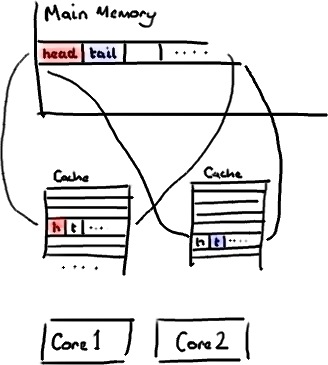
\includegraphics[width=0.65\textheight]{FalseSharing}
      \onslide<2>\centering
      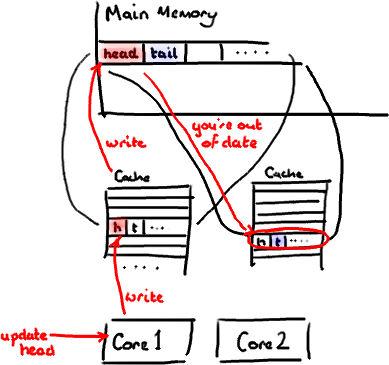
\includegraphics[width=0.7\textheight]{FalseSharingWriteHead}
      \onslide<3>\centering
      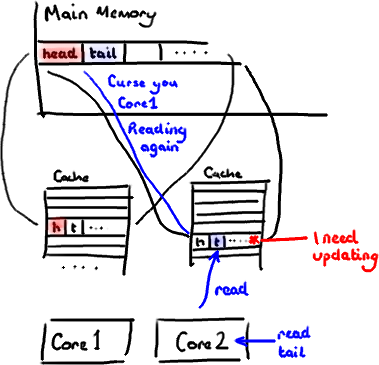
\includegraphics[width=0.7\textheight]{FalseSharingReadTail}
          \end{overprint}
    \caption{Example of cache misbehavior: {\bf False sharing}\\
      {\scriptsize By Trisha Gee, CC BY 3.0,
        \url{http://trishagee.github.io/post/dissecting_the_disruptor_why_its_so_fast_part_two__magic_cache_line_padding}}}
  \end{figure}
}

\frame{
  \frametitle{Supercomputers \& HPC Systems}

  \begin{description}
  \item[Monoprocessor with SIMD capabilities] ~
    \begin{itemize}
    \item Exploting the parallelism exposed:
      \begin{itemize}
      \item ILP
      \item SIMD: Vectorization
      \end{itemize}
    \item Also: Optimize memory hierarchy access
    \end{itemize}

    \pause

  \item[Shared memory multiprocessors] Processors share memory space
    \begin{itemize}
    \item Intra-node: easier programming model
    \item Exploting the parallelism exposed:
      \begin{itemize}
      \item Pthreads
      \item OpenMP
      \item Intel TBB
      \end{itemize}
    \end{itemize}

    \pause

  \item[Distributed memory multiprocessors] Processors have their own memory space
    \begin{itemize}
    \item Inter-node: (usually) harder programming
    \item Exploting the parallelism exposed:
      \begin{itemize}
      \item Message passing libraries: MPI, zeroMQ
      \item Data analytics frameworks (Big Data): Hadoop, Spark, Flink
      \end{itemize}
    \end{itemize}
  \end{description}
}

\frame{
  \frametitle{A Supercomputer: Finis Terrae II @CESGA}

   \begin{figure}
    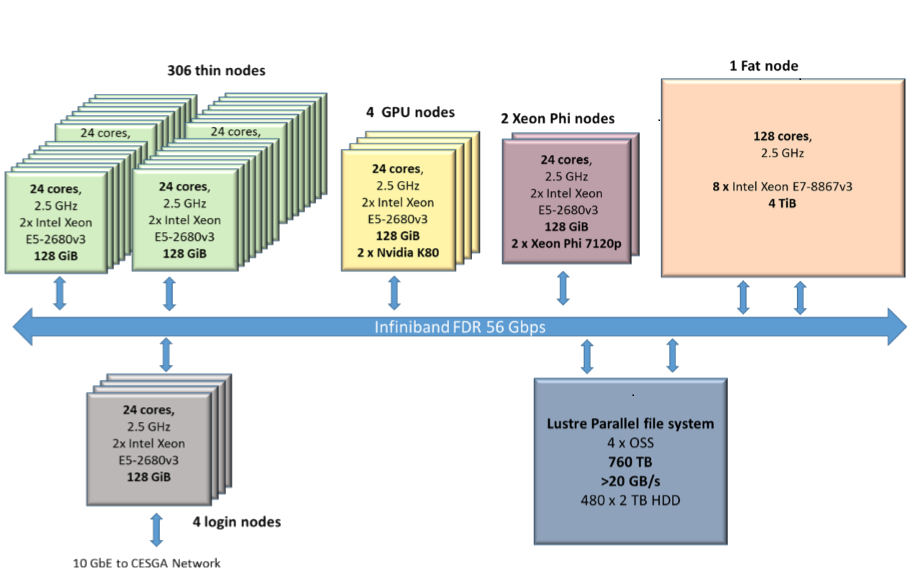
\includegraphics[width=\textwidth]{ftii}
    \caption{FT2 architecture}
  \end{figure}
}

\frame{
  \frametitle{FT2's compute nodes}

  \vspace*{-0.5cm}
  \begin{figure}
    \hspace*{-0.97cm}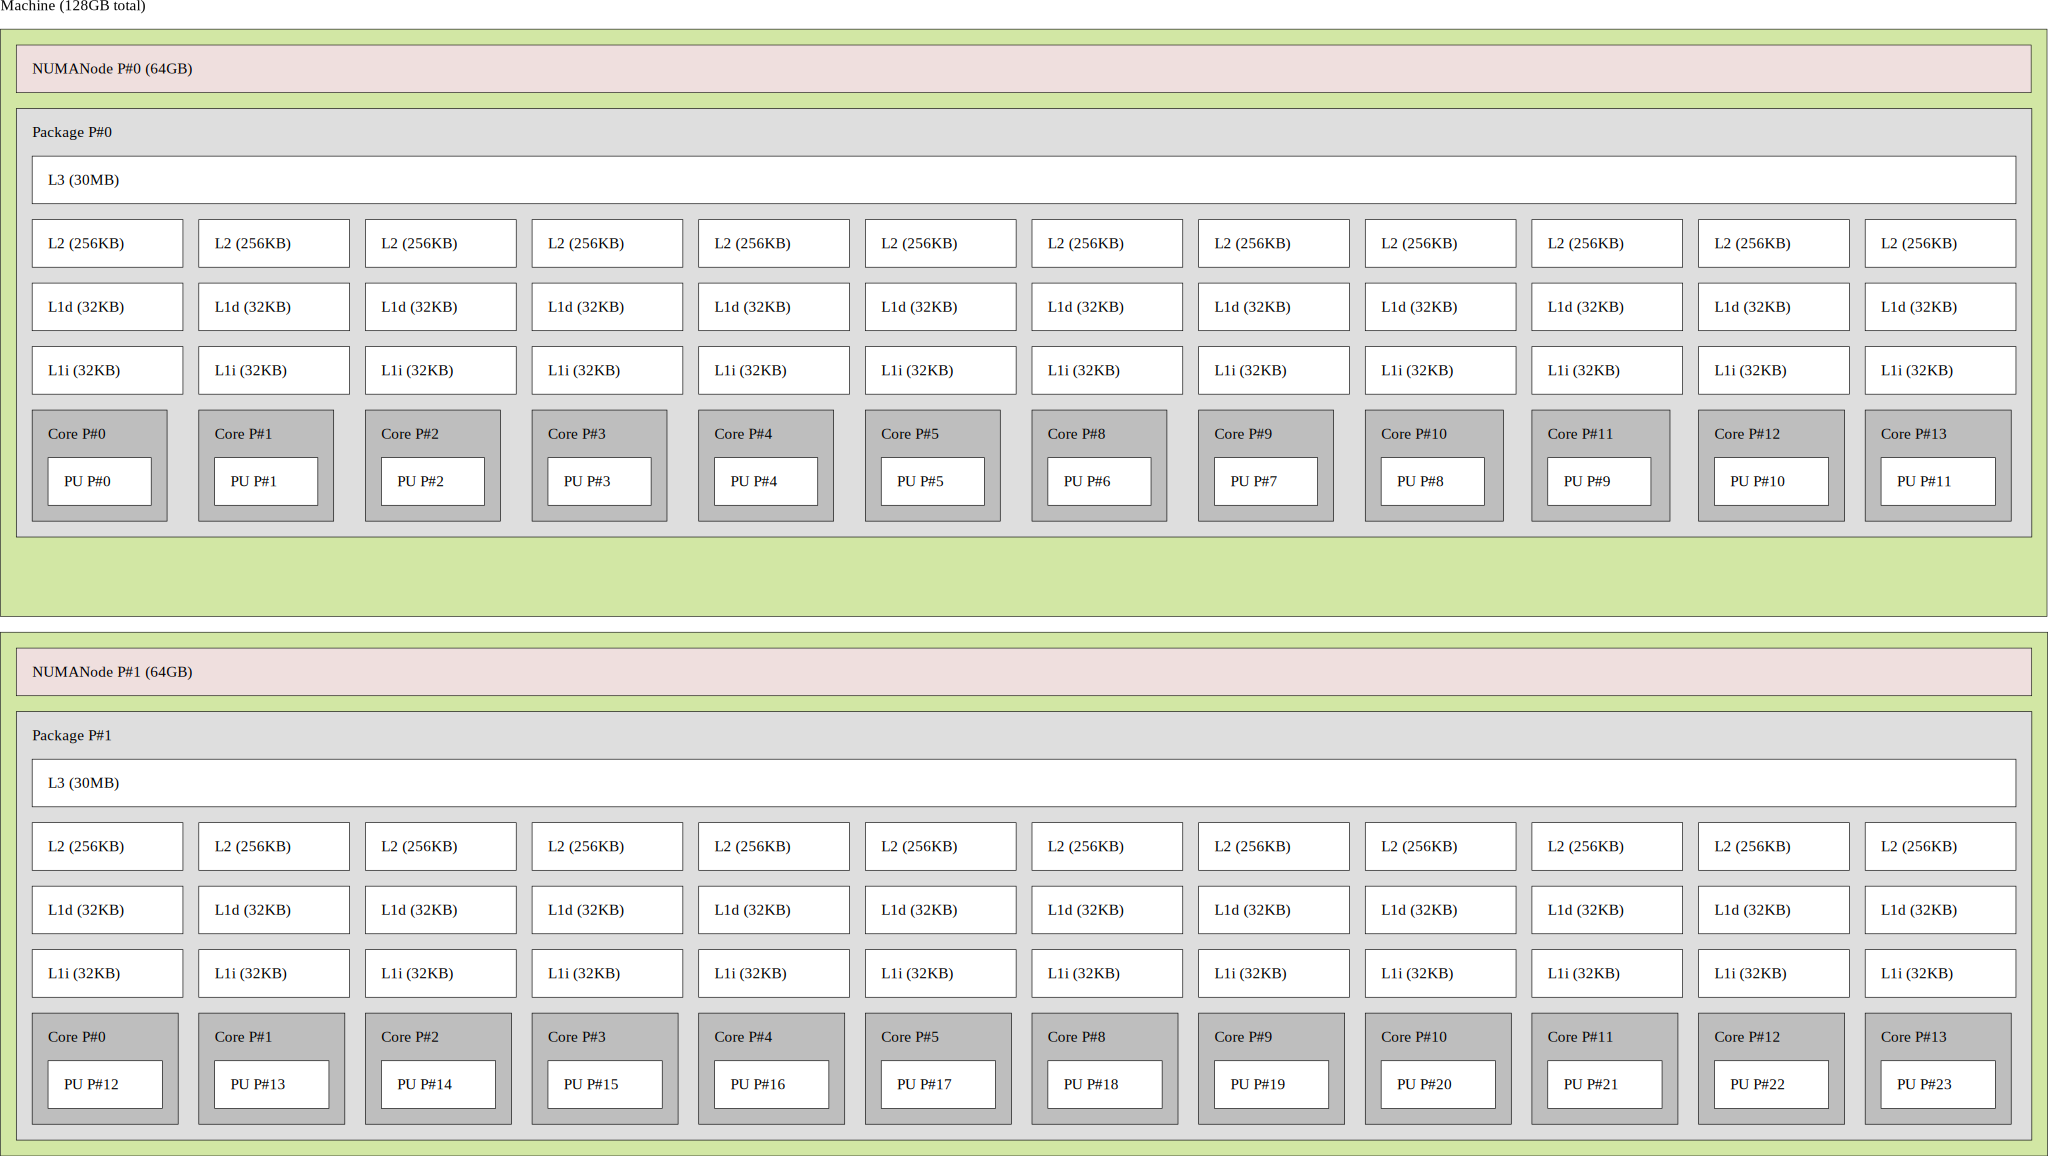
\includegraphics[width=1.18\textwidth]{ft2node}
    \caption{FT2 thin compute node}
  \end{figure}
}

\frame{
  \frametitle{Cache levels at FT2's nodes~\footnote{This and more info
    can be obtained in runtime with {\tt sysconf} (unistd.h) or with
    the command line utility {\tt getconf}}}

  \begin{description}
  \item[L1i]
    \begin{itemize}
    \item 32KB
    \item 8-way associative
    \item 64B/line
    \end{itemize}
  \item[L1d]
    \begin{itemize}
    \item 32KB
    \item 8-way associative
    \item 64B/line
    \end{itemize}
  \item[L2]
    \begin{itemize}
    \item 256KB
    \item 4-way associative
    \item 64B/line
    \end{itemize}
  \item[L3]
    \begin{itemize}
    \item 30MB
    \item 12-way associative
    \item 64B/line
    \end{itemize}
  \end{description}
}

\frame{
  \frametitle{Typical performance metrics}

  \begin{itemize}
  \item CPU
    \begin{itemize}
    \item MIPS
    \item FLOPS (usually GFLOPs/sec)
    \item Computational/Arithmetic intensity: FLOP/Byte
    \end{itemize}
  \item Memory \& I/O
    \begin{itemize}
    \item Latency (time units)
    \item Bandwith/Throutput (usually GBs/sec)
    \end{itemize}
  \item Cache
    \begin{itemize}
    \item Miss/Hit rate
    \end{itemize}
  \end{itemize}
}

\frame{
  \frametitle{Performance metrics for parallel applications}

  \begin{description}
  \item[Speedup:] Measure of performance
    \begin{itemize}
    \item Ratio between sequential and parallel execution times
      $$Speedup_{nprocs} = \frac{T_{seq}}{T_{nprocs}}$$
    \end{itemize}
  \item[Efficiency] Measure of use of computational resources
    \begin{itemize}
    \item Ratio between performance and resources used to achieve it
      $$Efficiency_{nprocs} = \frac{Speedup_{nprocs}}{nprocs} =
      \frac{T_{seq}}{nprocs \times T_{nprocs}}$$
    \end{itemize}
  \end{description}
}

\frame{
  \frametitle{Performance characterization}

  Identifying the dominant bottleneck:
  \begin{itemize}
  \item Compute bound (aka CPU bound)
  \item Memory bound
    \begin{itemize}
    \item Cache bound
    \end{itemize}
  \item I/O bound
  \end{itemize}

  Obviously, in terms of velocity:
  \begin{itemize}
  \item[] CPU > Cache (L1 > L2 > L3) > Mem > I/O
  \end{itemize}

}

% Good explanation from https://stackoverflow.com/questions/868568/what-do-the-terms-cpu-bound-and-i-o-bound-mean
% CPU Bound means the rate at which process progresses is limited by the speed of the CPU. A task that performs calculations on a small set of numbers, for example multiplying small matrices, is likely to be CPU bound.

% I/O Bound means the rate at which a process progresses is limited by the speed of the I/O subsystem. A task that processes data from disk, for example, counting the number of lines in a file is likely to be I/O bound.

% Memory bound means the rate at which a process progresses is limited by the amount memory available and the speed of that memory access. A task that processes large amounts of in memory data, for example multiplying large matrices, is likely to be Memory Bound.

% Cache bound means the rate at which a process progress is limited by the amount and speed of the cache available. A task that simply processes more data than fits in the cache will be cache bound.

% I/O Bound would be slower than Memory Bound would be slower than Cache Bound would be slower than CPU Bound.

% The solution to being I/O bound isn't necessarily to get more Memory. In some situations, the access algorithm could be designed around the I/O, Memory or Cache limitations.

\frame{
  \frametitle{The Roofline Model}

  \metroset{block=fill}

  \begin{block}{Basic Roofline Model}
    Bounds Floating-point performance as a function of
    \begin{itemize}
    \item machine peak performance (GFLOPs/sec)
    \item machine peak bandwidth (GBytes/sec)
    \item arithmetic intensity (FLOPs/Byte) \hfil \alert{\small $\leftarrow$ core concept}
    \end{itemize}
  \end{block}

  \begin{figure}
    \begin{overprint}
      \onslide<1>\centering
      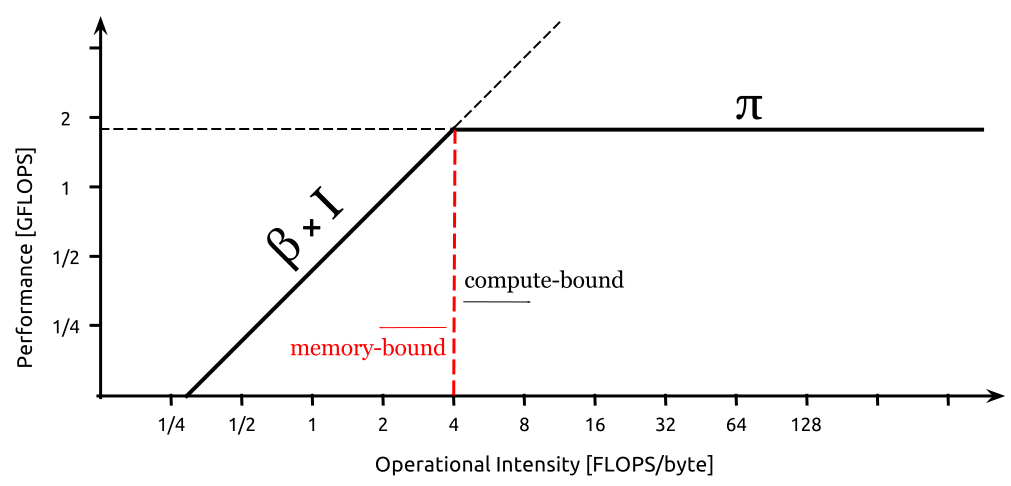
\includegraphics[width=.7\textwidth]{naive_roofline_model}
      \onslide<2>\centering
      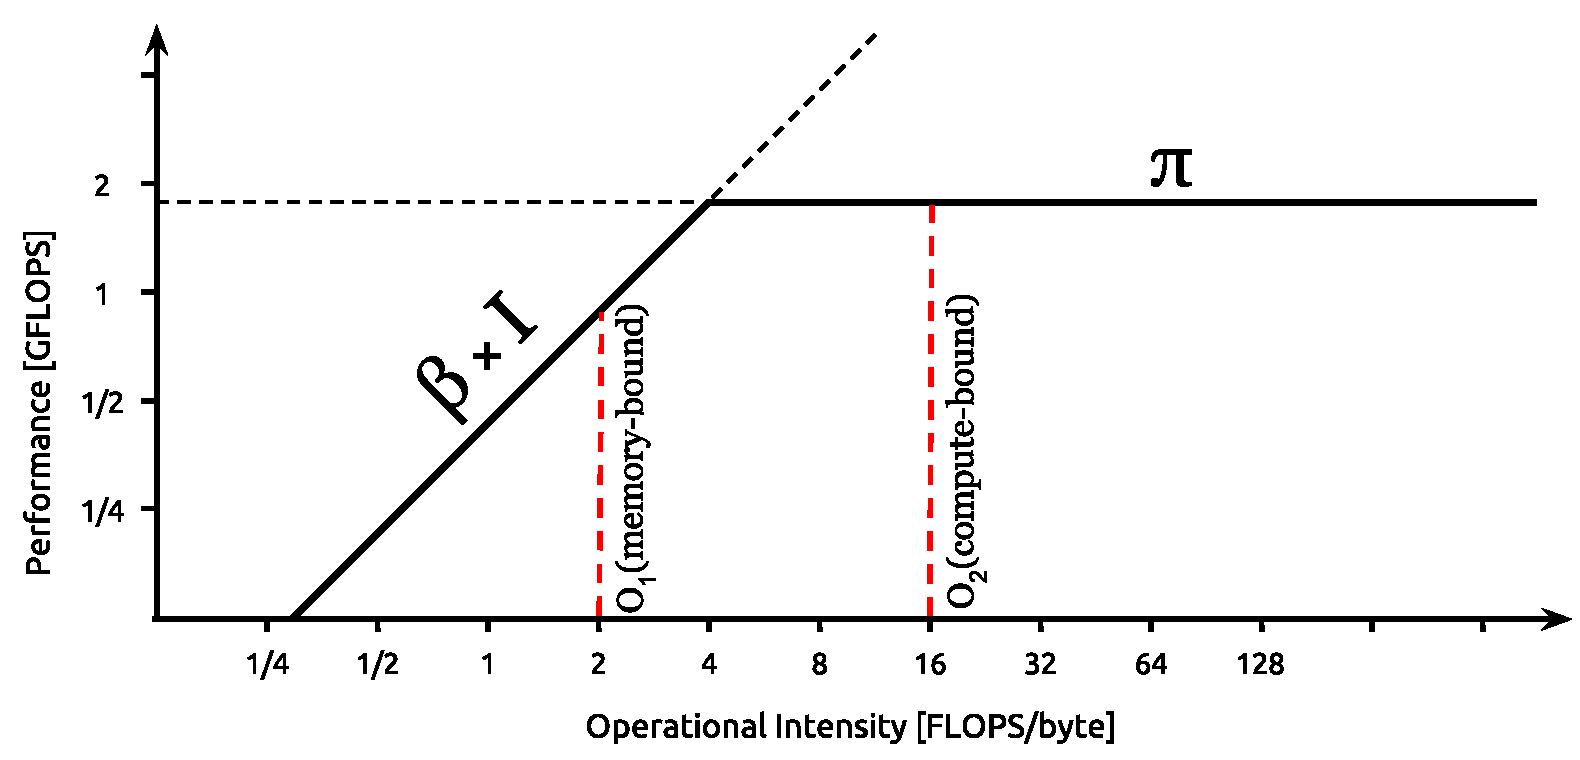
\includegraphics[width=.7\textwidth]{naive_roofline_model2}
    \end{overprint}
    \caption{Original image by Giu.natale, CC BY-SA 4.0, modified by me
      \url{https://commons.wikimedia.org/w/index.php?curid=49641351}}
  \end{figure}
}

\frame{
  \frametitle{Expanding the roofline plot}

  \begin{figure}\vspace*{-0.7cm}
    
\includegraphics[width=.5\textwidth]{roofline_model_bandwith_ceilings}~
    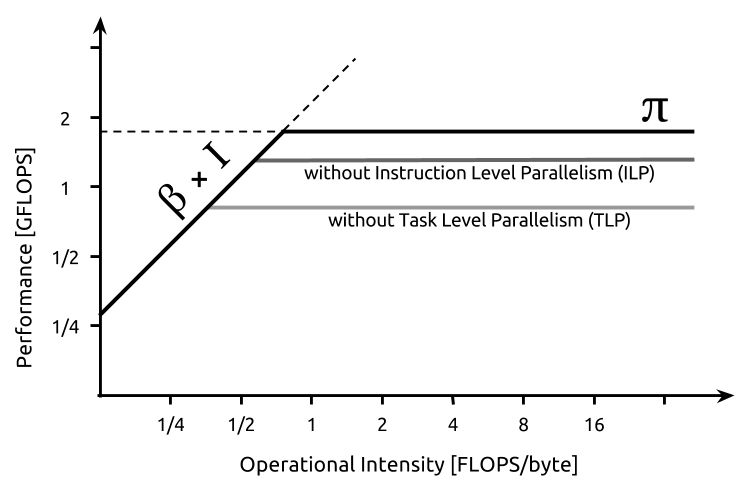
\includegraphics[width=.5\textwidth]{roofline_model_in-core_ceilings}
    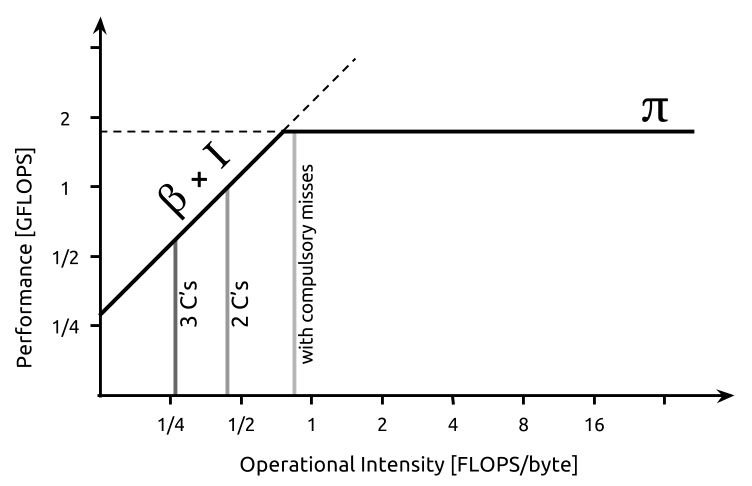
\includegraphics[width=.5\textwidth]{roofline_model_locality_walls}
    \caption{By Giu.natale - Own work, CC BY-SA 4.0,
      \url{https://commons.wikimedia.org/w/index.php?curid=49593615}
      \url{https://commons.wikimedia.org/w/index.php?curid=49593667}
      \url{https://commons.wikimedia.org/w/index.php?curid=49593835}
    }
  \end{figure}
}

\frame{
  \frametitle{Roofline model: an intuitive visual performance model}

  \begin{itemize}
  \item Provides performance estimation
    \begin{itemize}
    \item of a given compute kernel or application
    \item on a specific platform
    \end{itemize}

    \metroset{block=fill}
    \begin{block}{Visual and intuitive: key information at a glance}
      \begin{itemize}
      \item[\checkmark] Shows inherent hardware limitations
      \item[\checkmark] Highlights potential benefit and priority of
        optimizations
      \end{itemize}
    \end{block}
  \end{itemize}

  \begin{figure}
    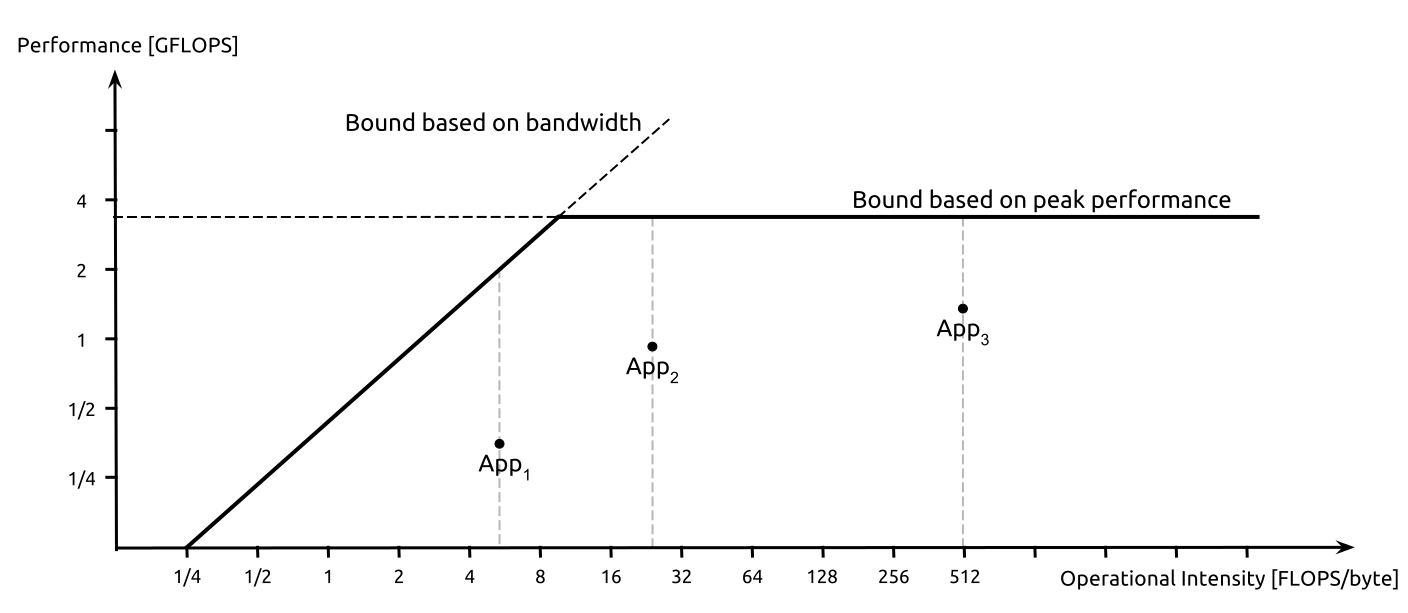
\includegraphics[width=.7\textwidth]{naive_roofline_model_example}
    \caption{By Giu.natale - Own work, CC BY-SA 4.0,
      \url{https://commons.wikimedia.org/w/index.php?curid=49641314}}
  \end{figure}
}



\section{Optimization and Profiling of (mainly) Sequential Code}

\frame{
  \frametitle{The art of computer programming: some
    \underline{keywords}}

  \begin{itemize}
  \item Code
  \item Compile
  \item Link
  \item Debug
  \item Profile
  \item Optimize
  \end{itemize}
}

\frame{
  \frametitle{\insertsectionhead}

  Main tools we'll use in this session:
  \begin{description}
  \item[Compiling] ~\\
    GNU Compilers: gcc, g++, gfortran
  \item[Debugging] ~\\
    gdb
  \item[Profiling and performance analysis] ~\\
    gprof, gcov, valgrind, gperftools
  \item[Performance characterization] ~\\
    Berkeley Lab's CS Roofline Toolkit
  \end{description}
}

\frame{
  \frametitle{Complementary tools}

  \setbeamertemplate{itemize subsubitem}[triangle]

  \begin{itemize}
  \item A good \emph{text editor} is essential to feel comfortable
    coding/debugging/profiling/optimizing
    \begin{itemize}
    \item I like {\tt emacs} (and {\tt vim} for other purposes)
    \end{itemize}

    \pause

  \item Terminal multiplexer: {\tt tmux} or {\tt screen}

    \pause

  \item System utilities/commands:
    \begin{description}
    \item[{\tt top}] (or htop\ldots)
    \item[{\tt pstack}] ~
    \item[{\tt ps}] and similars\ldots
    \end{description}
    \begin{itemize}
    \item I particularly like {\tt top}:
      \begin{itemize}
      \item see load per core: {\tt 1}
      \item toggling tasks/threads: {\tt H} ({\tt -H})
      \item filtering: {\tt o} (eg. {\tt COMMAND=mybinary})
      \item field management: {\tt f} (Last used CPU\ldots)
      \end{itemize}
    \end{itemize}

    \pause

  \item 
\includegraphics[width=2.5cm]{stackoverflow}
    \begin{itemize}
    \item \ldots and the rest of the Internet! (webs, chats, etc.)
    \end{itemize}
  \end{itemize}
}

\frame{
  \frametitle{Where are things in memory?}

  Something a (good) programmer should know to write efficient code:
  \begin{itemize}
  \item different \emph{``types of memory''}
  \item how variables are mapped to memory locations
  \end{itemize}
  \begin{figure}
    \includegraphics[width=0.8\textwidth]{memlayout}
    \caption{Program memory layout of Linux Executables}
  \end{figure}
}

\subsection{Compiler optimizations}

\frame{
  \frametitle{Looking at the compiler}
  How can the compiler help us to achieve efficient binaries from our
  source codes for a specific platform?
  \begin{itemize}
  \item Optimization options

    {\small \tt gcc [-Q] --help=optimizers}

    \makebox[0pt][r]{\tiny last gcc doc $\rightarrow$\hspace*{0.15cm}}{\scriptsize
      \url{http://gcc.gnu.org/onlinedocs/gcc/Optimize-Options.html}}

    \makebox[0pt][r]{\tiny gcc 6.4 doc $\rightarrow$\hspace*{0.15cm}}{\scriptsize
      \url{http://gcc.gnu.org/onlinedocs/gcc-6.4.0/gcc/Optimize-Options.html}}\\[0.5cm]

  \item Target-specific / machine-dependent options (x86)

    {\tt gcc [-Q] --help=target}

    \makebox[0pt][r]{\tiny last gcc doc $\rightarrow$\hspace*{0.15cm}}{\scriptsize
      \url{http://gcc.gnu.org/onlinedocs/gcc/x86-Options.html}}

    \makebox[0pt][r]{\tiny gcc 6.4 doc $\rightarrow$\hspace*{0.15cm}}{\scriptsize
      \url{http://gcc.gnu.org/onlinedocs/gcc-6.4.0/gcc/x86-Options.html}}
  \end{itemize}
  }

\frame{
  \frametitle{Compiler machine-dependent options (x86)}

  (a.k.a. {\it `-m'} options)

  \begin{description}
  \item[{\tt -march={\it cpu-type}}] Generate instructions for that
    machine type\\
    E.g. {\tt native|x86-64|haswell|\ldots}
  \item[{\tt -mtune={\it cpu-type}}] Tune generated code for that
    machine type
  \item[{\tt -mavx -mavx2\ldots}] Enable the use of extended
    instruction sets (vector instructions, mostly)
  \end{description}

  \vfill
  $\rightarrow$ {\footnotesize Check target specific options with:
    {\tt gcc -Q -march=native --help=target}}
}

\frame{
  \frametitle{Compiler optimization levels}

  In a nutshell: \hfil (each level includes the previous)
  \begin{description}
  \item[{\tt -O0}] [Default] No optimization. Reduces compilation time
    and make debugging produce the expected results.
  \item[{\tt -O/-O1}] Optimize. Tries to reduce code size and execution
    time, avoiding optimizations that take high compilation time.
  \item[{\tt -O2}] Optimizes even more.
  \item[{\tt -O3}] Optimizes yet more.
  \item[{\tt -Ofast}] Enables {\tt -ffast-math}, optimizations that
    are not valid for all standard-compliant programs.

    Additionally, Fortran-specific {\tt -fstack-arrays}, unless {\tt
      -fmax-stack-var-size} is specified, and {\tt
      -fno-protect-parens}.
  \end{description}

  $\rightarrow$ {\footnotesize Check specific options being enable/disable at
    each level for your compiler version with {\tt gcc -Q -O2
      --help=optimizers} (or in the doc)}
}

\frame{
  \frametitle{Compiling to debug and/or profile a code}

  Compiling to debug, basically:
  \begin{description}
  \item[{\tt -g}] Includes extra information to use by a debugger\\
    Typically used together with {\tt -O0} (no optimizations)
  \item[{\tt -Og}] Optimize debugging experience: enables
    optimizations that do not interfere with debugging
  \item[$\Rightarrow$] More fine tuning options in the doc
    
    \makebox[0pt][r]{\tiny last gcc doc $\rightarrow$\hspace*{0.15cm}}{\scriptsize
      \url{http://gcc.gnu.org/onlinedocs/gcc/Debugging-Options.html}}

    \begingroup
    \leftskip0em
    \rightskip\leftskip
    \makebox[0pt][r]{\tiny gcc 6.4 doc $\rightarrow$\hspace*{0.15cm}}{\scriptsize
      \url{http://gcc.gnu.org/onlinedocs/gcc-6.4.0/gcc/Debugging-Options.html}}
    \par
    \endgroup
  \end{description}

  \pause
  
  Compiling to profile (instrumentation options):
  \begin{description}
  \item[{\tt -pg}] Generate extra code to write profile information
    for {\tt gprof}
  \item[$\Rightarrow$] More fine tuning options in the doc
    
    \makebox[0pt][r]{\tiny last gcc doc $\rightarrow$\hspace*{0.15cm}}{\scriptsize
      \url{http://gcc.gnu.org/onlinedocs/gcc/Instrumentation-Options.html}}

    \begingroup
    \leftskip0em
    \rightskip\leftskip
    \makebox[0pt][r]{\tiny gcc 6.4 doc $\rightarrow$\hspace*{0.15cm}}{\scriptsize
      \url{http://gcc.gnu.org/onlinedocs/gcc-6.4.0/gcc/Instrumentation-Options.html}}
    \par
    \endgroup
  \end{description}
}

\begin{frame}[fragile]{Other interesting compiler options}

  \begin{itemize}
  \item I like to activate all relevant \emph{warnings}: {\tt -Wall
      -Wextra}
  \item Use {\tt -D} to pass macros used in the code to precompiler

    \pause

  \item Generate ASM code \emph{``easy to read''} (eg. to check
    vectorization)
        \begin{lstlisting}[style=shell,gobble=5,caption={From the book
\emph{Algorithms for programmers}\footnote<2>{Algorithm for programmers:
\url{https://www.jjj.de/fxt/fxtbook.pdf}}\footnote<2>{Generating Mixed
Source and Assembly List using GCC: {\scriptsize \url{http://www.systutorials.com/240/generate-a-mixed-source-and-assembly-listing-using-gcc}}}}]
         # create assembler code:
         c++ -S -fverbose-asm -g -O2 test.cc -o test.s

         # create asm interlaced with source lines:
         as -alhnd test.s > test.lst
       \end{lstlisting}
  \end{itemize}

\end{frame}

\frame{
  \frametitle{Some key optimizations at compilation~\footnote{\ldots or at
      \emph{coding time}, some of them} time}

  \begin{itemize}
  \item Use registers
  \item Inlining
  \item Reduce and improve conditionals
  \item Loop optimizations
    \begin{itemize}
    \item Loop unrolling
    \item Loop peeling
    \end{itemize}
  \item Memory data layout
    \begin{itemize}
    \item Mem alignment
    \item Aliasing
    \end{itemize}
  \item Prefetching
  \item Interprocedural optimizations
  \item Profile-guided optimizations (PGO)
  \item Vectorization
  \end{itemize}
}

\begin{frame}[fragile]{Vectorization}

  \begin{description}
  \item[Vectorization] Form of SIMD which allows us to crunch multiple
    values in one CPU instruction
  \end{description}

  $\Rightarrow$ Especially useful to \underline{optimize loop execution} (but not
  exclusively)

  \begin{columns}
    \column{0.45\textwidth}{
      \begin{lstlisting}[style=c,gobble=8,caption={Sequential loop}]
        float A[32], B[32], C[32];

        for (i=0; i<32; i++)
          C[i] = A[i] + B[i];
          // 32 float ADD ops
      \end{lstlisting}
    } \
    \column{0.55\textwidth}{
      \begin{lstlisting}[style=c,gobble=8,caption={Vectorized pseudocode}]
        float A[32], B[32], C[32];

        for (i=0; i<32; i+=8)
          C[i:i+7] = A[i:i+7] + B[i:i+7];
          // vectorization factor: 8
          // => 4 vector float ADD ops
      \end{lstlisting}
    }
  \end{columns}
\end{frame}

\frame{
  \frametitle{Vectorization: Intel SIMD extensions}

  \begin{figure}
    \includegraphics{avx_regs}
    \caption{x86-64 Vector Registers}
  \end{figure}
  \begin{itemize}
  \item AVX-512 (ZMM0--ZMM31)
  \item AVX/AVX2 (YMM0--YMM31) \quad \alert{\small $\rightarrow$ AVX2 in FT2's Haswell procs}
  \item SSE (XMM0--XMM31)
  \end{itemize}
}

\begin{frame}[fragile]{Vectorization: x86-64 vector operations}

  \begin{itemize}
  \item Intrinsic C-like functions to access vector instructions\\
    e.g.\\[0.2cm]
    \begin{columns}
      \column{0.33\textwidth}{
        {\bf AVX asm instruction}\\
        \begin{lstlisting}[style=asm,gobble=9]
          vmovaps ymm, m256
        \end{lstlisting}
      } \
      \column{0.77\textwidth}{
        {\bf Intrinsic function}\\
        \begin{lstlisting}[style=c,gobble=9]
          __m256 _mm256_load_ps (float const *mem_addr)
          #include <immintrin.h>
        \end{lstlisting}
      }
    \end{columns}

  \item[] \hspace*{-0.7cm} \mbox{\scriptsize \alert{(doc)} Intrinsics Guide: \url{http://software.intel.com/sites/landingpage/IntrinsicsGuide}}\\[0.2cm]
  \item SIMD instructions typically require:
    \begin{itemize}
    \item aligned data
    \item no pointer aliasing\\
      {\small (pointers are aliased if they can refer to same storage location)}
    \end{itemize}
  \end{itemize}

  \pause

  \begin{columns}
    \column{0.35\textwidth}{
      \begin{alertblock}{Writing vectorized code}
        \begin{itemize}
        \item hard
        \item error-prone
        \end{itemize}
      \end{alertblock}
    }
    \column{0.01\textwidth}{
      \mbox{$\Rightarrow$}
    }
    \column{0.5\textwidth}{
      \begin{exampleblock}{Autovectorization}
        \structure{\checkmark} Let compiler do it for you\\
        \pause
        {\small $\rightarrow$ Sometimes, compiler needs some help, though}
      \end{exampleblock}
    }
  \end{columns}
\end{frame}


\frame{
  \frametitle{GCC autovectorization compiler flags}

  \begin{description}
  \item[{\tt -ftree-loop-vectorize}] Enable loop vectorization
  \item[{\tt -ftree-slp-vectorize}] Enable basic block vectorization (SLP)
  \end{description}
  \begin{itemize}
  \item Both flags are enabled by default in {\tt -O3} and {\tt
      -Ofast}, and are also enabled with {\tt -ftree-vectorize}
  \item {\tt Ofast}'s additional (unsafe) math optims may help autovect
  \item Do not forget {\tt -march=native}
  \item Reports: list (not) vectorized loops + extra info
    {\tt -fopt-info-vec}\\
    {\tt -fopt-info-vec-missed}\\
    {\tt -fopt-info-vec-all} {\footnotesize(detailed autovect process)}
  % \item Additionally:
  %   \begin{description}
  %   \item[{\tt -fvect-cost-model=[unlimited|dynamic|cheap]}] Specifies
  %     the cost model for vectorization
  %     %(default O3/Ofast: {\tt dynamic})
  %   \item[{\tt -fsimd-cost-model=[unlimited|dynamic|cheap]}] Specifies
  %     the vectorization cost model for code marked with a simd
  %     directive
  %     %(default O3/Ofast: {\tt unlimited})
  % \end{description}
  \end{itemize}
}

\frame{
  \frametitle{GCC autovectorization: compiler directives and C keywords}

  GCC Vectorization
  pragmas~\footnote{\url{http://gcc.gnu.org/onlinedocs/gcc/Loop-Specific-Pragmas.html}}:
  \begin{itemize}
  \item {\tt \#pragma GCC ivdep}
    \begin{itemize}
    \item programmer asserts no loop-carried dependencies
    \end{itemize}
  \end{itemize}

  C keywords:
  \begin{itemize}
  \item {\tt restrict}~\footnote{\url{http://en.wikipedia.org/wiki/Restrict}}
    \begin{itemize}
    \item used in pointer declarations to assert there's no aliasing
    \end{itemize}
  \end{itemize}
}

\frame{
  \frametitle{Vectorization: requirements and limitations}

  \begin{itemize}
  \item Countable loops
  \item No backward loop-carried dependencies
  \item No function calls
    \begin{itemize}
    \item Except vectorizable math functions e.g. sin, sqrt,\ldots
    \end{itemize}
  \item Straight-line code (only one control flow: no switch)
  \item Loop to be vectorized must be innermost loop if nested
  \end{itemize}
}

\frame{
  \frametitle{Profile-guided optimization (PGO)}

  \begin{enumerate}
  \item {\bf First compilation phase}: Instrument the application with profiling code
    \begin{itemize}
    \item[$\rightarrow$] application will log profiling data when running
    \end{itemize}
  \item {\bf Execute the instrumented binary}
    \begin{itemize}
    \item[$\rightarrow$] profiling files are generated for each run
    \end{itemize}
  \item {\bf Second compilation phase}: Rebuild the application to
    leverage profiling data to optimize it
  \end{enumerate}
}

\frame{
  \frametitle{Profile-guided optimization (PGO) in gcc}

  \begin{description}
  \item[{\tt -fprofile-generate}] enables \begin{itemize}
    \item[] {\tt -fprofile-arcs}
    \item[] {\tt -fprofile-values}
    \item[] {\tt -fvpt}
    \end{itemize}
  \end{description}
  \begin{enumerate}
  \item A {\tt .gcno} file is generated for each object file
    \begin{itemize}
    \item these files are also used for {\tt gcov} coverage reports
    \end{itemize}
  \item Then, multiple executions record coverage data into .gcda
    files
  \item Finally, recompile with {\tt -fprofile-use}
    \begin{itemize}
    \item gathers the coverage data and infer if a branch is
      likely/unlikely
    \end{itemize}
  \item[$\rightarrow$] Resulting binary will be better at prefetching code
  \end{enumerate}
  \begin{description}
  \item[{\tt -fprofile-use}] enables \begin{itemize}
    \item[] {\tt -fbranch-probabilities}
    \item[] {\tt -fvpt}
    \item[] {\tt -funroll-loops}
    \item[] {\tt -fpeel-loops}
    \item[] {\tt -ftracer}
    \end{itemize}
  \end{description}
}



\subsection{Profiling: Evaluate execution time and detect hot spots}

\frame{
  \frametitle{Profile first, optimize later}

  \begin{quote}
    Premature optimization is the root of all evil -- {Donald Knuth}
  \end{quote}
}

\frame{
  \frametitle{Profiling}

  \metroset{block=fill}
  \begin{block}{Why to profile?}
    \begin{itemize}
    \item Evaluate performance
    \item Find the performance bottlenecks
      \begin{itemize}
      \item inefficient programming / bugs
      \item memory and I/O bottlenecks
      \item parallel scaling
      \end{itemize}
    \end{itemize}
  \end{block}

  \begin{itemize}
  \item Profiling tools help you analyze your code's performance:
    \begin{itemize}
    \item how often each line of code executes
    \item what lines of code are actually executed
    \item how much computing time each section of code uses
    \end{itemize}
  \end{itemize}

  \begin{itemize}
  \item 2 main approaches:
    \begin{itemize}
    \item Instrumenting profiler
    \item Sampling profiler
      \begin{itemize}
      \item hardware counters
      \item system information
      \end{itemize}
    \end{itemize}
  \end{itemize}
}

\begin{frame}[fragile]{First approach: self-profiling!}

  \begin{itemize}
  \item Insert explicit \emph{timestamps} in your code
    \begin{itemize}
    \item DIY instrumentation
    \item Most common approach when you're writing your own code
      \begin{itemize}
      \item you know the structure/flow $\Rightarrow$ where to measure
      \end{itemize}
    \end{itemize}

    \pause

  \item In C, I like the function {\tt gettimeofday()}
    \begin{itemize}
    \item microseconds precision
    \end{itemize}

    \begin{lstlisting}[style=c,gobble=4]
      #include <sys/time.h>

      int gettimeofday(struct timeval *tv, struct timezone *tz)
   \end{lstlisting}

    \begin{lstlisting}[style=c,gobble=4]
      <sys/time.h>

      struct timeval {
          time_t      tv_sec;   /* seconds */
          suseconds_t tv_usec;  /* microseconds */
      };
      struct timezone {
          int tz_minuteswest;   /* minutes west of Greenwich */
          int tz_dsttime;       /* type of DST correction */
      };
   \end{lstlisting}
  \end{itemize}

\end{frame}

\frame{
  \frametitle{GPROF: the GNU Profiler}

  \begin{overprint}
    {\bf Gprof}: performance analysis tool for Unix applications, part of
    binutils\footnote{\url{http://www.gnu.org/software/binutils}}
    \begin{itemize}
    \item hybrid (compiler assisted) \emph{instrument.} and
      \emph{sampling} approach
    \end{itemize}

    How to use it:
    \begin{enumerate}
    \item Have profiling enabled while compiling the code
      \uncover<2->{
        \begin{itemize}
        \item[$\rightarrow$] gcc profiling flag: {\tt -pg}
        \end{itemize}
      }
    \item Execute the program code to produce the profiling data
      \uncover<2->{
        \begin{itemize}
        \item[$\rightarrow$] {\tt gmon.out} archive is generated
        \end{itemize}
      }
    \item Run the gprof tool on the profiling data file (generated in
      the step above)
      \uncover<2->{
        \begin{itemize}
        \item[{\tt \$}] {\tt gprof program\_binary [gmon.out]}
        \end{itemize}
      }
    \end{enumerate}

    \onslide<3>
    \vfill
    What GPROF provides:
    \begin{itemize}
    \item Flat profile
    \item Call graph
    \end{itemize}
    \quad
  \end{overprint}
}

\begin{frame}[fragile]{GPROF: Flat profile}

  \begin{block}{Flat Profile}
    \begin{itemize}
    \item Time spent executing each function {\small (sampled
        $\Rightarrow$ statistical inac.)}
    \end{itemize}
  \end{block}

  \begin{lstlisting}[gobble=3, caption={Flat profile example}]
    Each sample counts as 0.01 seconds.
      %   cumulative   self              self     total
     time   seconds   seconds    calls  ms/call  ms/call  name
     33.34      0.02     0.02     7208     0.00     0.00  open
     16.67      0.03     0.01      244     0.04     0.12  offtime
     16.67      0.04     0.01        8     1.25     1.25  memccpy
     16.67      0.05     0.01        7     1.43     1.43  write
     16.67      0.06     0.01                             mcount
      0.00      0.06     0.00      236     0.00     0.00  tzset
      0.00      0.06     0.00      192     0.00     0.00  tolower
      0.00      0.06     0.00       47     0.00     0.00  strlen
      0.00      0.06     0.00       45     0.00     0.00  strchr
      0.00      0.06     0.00        1     0.00    50.00  main
      0.00      0.06     0.00        1     0.00     0.00  memcpy
      0.00      0.06     0.00        1     0.00    10.11  print
      ...
  \end{lstlisting}

\end{frame}

\begin{frame}[fragile]{GPROF: Call graph}

  \begin{block}{ Call Graph}
    \begin{itemize}
    \item Time spent in each function and its children
    \end{itemize}
  \end{block}

  \begin{lstlisting}[gobble=3, basicstyle=\scriptsize\ttfamily, caption={Call graph example}]
    granularity: each sample hit covers 2 byte(s) for 20.00% of 0.05 seconds

    index % time    self  children    called     name
                                                     <spontaneous>
    [1]    100.0    0.00    0.05                 start [1]
                    0.00    0.05       1/1           main [2]
                    0.00    0.00       1/2           on_exit [28]
                    0.00    0.00       1/1           exit [59]
    -----------------------------------------------
                    0.00    0.05       1/1           start [1]
    [2]    100.0    0.00    0.05       1         main [2]
                    0.00    0.05       1/1           report [3]
    -----------------------------------------------
                    0.00    0.05       1/1           main [2]
    [3]    100.0    0.00    0.05       1         report [3]
                    0.00    0.03       8/8           timelocal [6]
                    0.00    0.01       1/1           print [9]
                    0.00    0.01       9/9           fgets [12]
                    0.00    0.00      12/34          strncmp <cycle 1> [40]
                    0.00    0.00       8/8           lookup [20]
                    0.00    0.00       1/1           fopen [21]
                    0.00    0.00       8/8           chewtime [24]
                    0.00    0.00       8/16          skipspace [44]
    -----------------------------------------------
    [4]     59.8    0.01        0.02       8+472     <cycle 2 as a whole> [4]
                    0.01        0.02     244+260         offtime <cycle 2> [7]
                    0.00        0.00     236+1           tzset <cycle 2> [26]
    -----------------------------------------------
  \end{lstlisting}
\end{frame}

\frame{
  \frametitle{GPROF: some useful parameters}

  \begin{description}
  \item[{\tt -s}] combine the data from several runs to minimize
    statistical inaccuracy in measures
  \item[{\tt -a}] suppress the printing of statically declared
    (private) functions
  \item[{\tt -b}] suppress verbose blurbs
  \item[{\tt -pfunct\_name}] flat profile for a specific function
  \item[{\tt -qfunct\_name}] call graph for a specific function
  \end{description}
}

\begin{frame}[fragile]{Gprof and gprof2dot}

  \begin{block}{gprof2dot}
    Python script to convert output from many profilers into a dot graph
  \end{block}

  \begin{lstlisting}[gobble=3]
    gprof program\_binary [gmon.out] | gprof2dot.py \
                                     | dot -Tpng -o output.png
  \end{lstlisting}

  \begin{figure}
    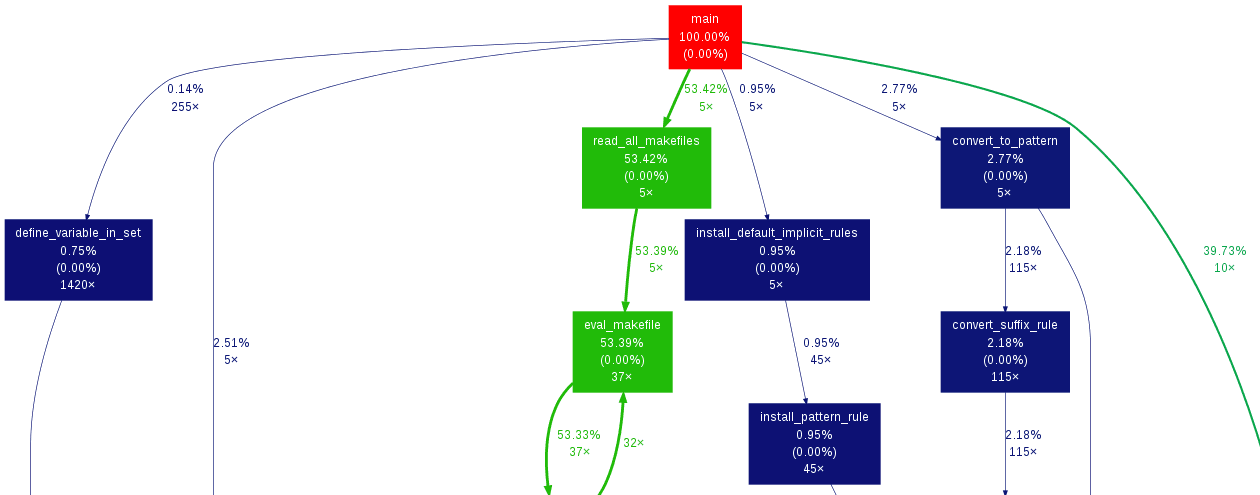
\includegraphics{gprof2dot_ex}
  \end{figure}

  \begin{columns}
    \column{.45\textwidth}{
      \begin{exampleblock}{Requirements}
        $\text{Python2} \geq 2.7$ or $\text{Python3} \geq 3.3$\\
        Graphviz
      \end{exampleblock}
    }
    \column{.6\textwidth}{
      \begin{alertblock}{Source \& pip package}
        {\footnotesize \url{http://github.com/jrfonseca/gprof2dot}}\\
        {\footnotesize \tt \$~pip install gprof2dot}
      \end{alertblock}
    }
  \end{columns}
\end{frame}

\frame{
  \frametitle{Gprof: caveats}

  GPROF main drawbacks:
  \begin{itemize}
  \item Relatively high overhead (mainly caused by instrumentation)
  \item Does not support profiling multi-threaded applications!
    \begin{itemize}
    \item there are some workarounds\ldots~\footnote{\mbox{gprof \& multithreaded code: {\scriptsize
      \url{http://sam.zoy.org/writings/programming/gprof.html}}}
  }~\footnote{gprof
        \& MPI: {\scriptsize \url{http://shwina.github.io/2014/11/profiling-parallel}}}
    \end{itemize}
  \item Cannot profile shared libraries
  \item Blind to I/O
  \item Other unexpected/weird behaviors
  \end{itemize}
}

\frame{
  \frametitle{Valgrind: a swiss army knife tool~\footnote{\url{http://valgrind.org}}}

  {\bf Valgrind:} instrumentation \underline{framework} for building
  analysis tools
  \begin{itemize}
  \item Typical use:
    \begin{itemize}
    \item debugging: detect memory management and threading bugs
    \item profiling: cache, mem, branches\ldots
    \end{itemize}
  \item ... but you can also use Valgrind to build your own tool!
  \end{itemize}

  \begin{block}{Valgrind is basically a virtual machine}
  \begin{itemize}
  \item[$\rightarrow$] just in time recompilation of x86 machine code
    to some simpler RISC-like intermediate code: UCode
  \item[$\rightarrow$] depending on the chosen tool, UCode is instrumented appropriately to record the data of interest
  \end{itemize}
  \end{block}
}

\frame{
  \frametitle{Valgrind: tools provided}

  6 tools included in current versions:
  \begin{description}
  \item[Memcheck:] a memory error detector
  \item[Callgrind:] a code profiler
  \item[Cachegrind:] a cache and branch-prediction profiler
  \item[Helgrind and DRD:] two different thread error detectors
  \item[Massif:] a heap profiler
  \end{description}

  Also, 3 experimental tools:
  \begin{itemize}
  \item a stack/global array overrun detector: {\bf SGCheck}
  \item another dynamic heap profiler: {\bf DHAT}
  \item a SimPoint basic block vector generator: {\bf BBV}
  \end{itemize}
}

\begin{frame}[fragile]{Valgrind: detecting memory-related errors with
    Memcheck}

  \begin{description}
  \item[Memcheck:] The default tool, and the most popular
    \begin{itemize}
    \item[\checkmark] Easy way to detect and locate memory bugs
    \item[{\tt x}] Main drawback: it is {\bf slow!} (Valgrind, in general)
    \item[{\tt x}] Second main drawback: some false positives!
    \end{itemize}
  \end{description}

  \pause

  How to use it?
  \begin{itemize}
  \item Compile your code with {\tt -g} (debugging symbols
    $\Rightarrow$ line numbers)
  \item Maybe a good idea to limit compiler opts: {\tt -O0 or -O1}
  \item Launch detailed memory leak detector ({\tt --leak-check=yes}):
    \begin{lstlisting}
      valgrind --leak-check=yes myprog arg1 arg2
    \end{lstlisting}
  \item Read the (verbose) output!
  \end{itemize}

  \pause

  \begin{exampleblock}{Objective}
    Try to make your program so clean that Memcheck reports no errors
  \end{exampleblock}
\end{frame}

\begin{frame}[fragile]{Valgrind: Memcheck example}

  \begin{lstlisting}[gobble=2]
    #include <stdlib.h>

    void f(void) {
      int *x = malloc(10 * sizeof(int));
      x[10] = 0;     // problem 1: heap block overrun
    }                // problem 2: memory leak -- x not freed

    int main(void) {
      f();
      return 0;
    }
  \end{lstlisting}

  \vspace*{-0.5cm}%
  \hspace{-0.6cm}%
  \begin{overprint}
    \onslide<1>
    \begin{lstlisting}[style=valgrind,gobble=6,caption={Valgrind output: Memcheck error}]
      ==19182== Invalid write of size 4
      ==19182==    at 0x804838F: f (example.c:6)
      ==19182==    by 0x80483AB: main (example.c:11)
      ==19182==  Address 0x1BA45050 is 0 bytes after a block of size 40 alloc'd
      ==19182==    at 0x1B8FF5CD: malloc (vg_replace_malloc.c:130)
      ==19182==    by 0x8048385: f (example.c:5)
      ==19182==    by 0x80483AB: main (example.c:11)
    \end{lstlisting}

    \onslide<2>
    \begin{lstlisting}[style=valgrind,gobble=6,
      caption={Valgrind output: Memory leaks messages}]
      ==19182== 40 bytes in 1 blocks are definitely lost in loss record 1 of 1
      ==19182==    at 0x1B8FF5CD: malloc (vg_replace_malloc.c:130)
      ==19182==    by 0x8048385: f (a.c:5)
      ==19182==    by 0x80483AB: main (a.c:11)
    \end{lstlisting}
  \end{overprint}

\end{frame}

\frame{
  \frametitle{Valgrind: Memcheck memory leaks report}

  Memcheck classifies memory leaks in 4 general types:
  \begin{description}
  \item[Still reachable] Not specially relevant
  \item[Definitely lost] Symptom of problems. This is a
    \underline{memory leak}
  \item[Indirectly lost] Problems usually caused by a previous
    definitely lost issue (that should be fixed earlier!)
  \item[Possibly lost] Inner pointers to allocated mem
    blocks. Investigate if not on purpose
  \end{description}

  \pause

  \begin{exampleblock}{Personally\ldots}
    I like achieving {\bf memcheck-clean} runs
  \end{exampleblock}
}

\frame{
  \frametitle{Valgrind: Memcheck can be used in parallel environments}

  \begin{itemize}
  \item {\bf Memcheck} can be used to debug and profile parallel
    programs: \emph{pthreads}, \emph{openmp}, even \emph{MPI}!
    \begin{itemize}
    \item usually increases the number of false positives!
    \end{itemize}
  \item Very good documentation: {\small \url{http://valgrind.org/docs/manual/mc-manual.html}}
  \end{itemize}
}

\frame{
  \frametitle{Valgrind: performance profiling with Callgrind}

  \begin{description}
  \item[Callgrind:] a profiling tool that records the function call history as a call-graph
    \begin{itemize}
    \item[\checkmark] Simple way of creating a CPU profile of your
      application
    \item[{\checkmark}] The profiling result is {\bf not} influenced by the
      measurement.
    \item[{\tt x}] Again: terribly slow!
    \end{itemize}
  \end{description}

  \pause

  \begin{itemize}
  \item 2 post-mortem analysis tools:
    \begin{itemize}
    \item Command line: {\tt callgrind\_annotate}
    \item Great visualizatoin tool to help us to interpretate
      collected data: {\tt KCachegrind}
    \end{itemize}
  \item One interactive command line tool to control execution:
    {\small \tt
      callgrind\_control}
  \end{itemize}
}

\begin{frame}[fragile]{Valgrind: Callgrind typical use}

  How to use it?~\footnote{Windows binary (I dit not test it):
    \url{http://sourceforge.net/projects/qcachegrindwin}}
  \begin{itemize}
  \item Compile your code with {\tt -g} (debugging symbols
    $\Rightarrow$ line numbers)
  \item Launch cachegrind:
    \begin{lstlisting}
      valgrind --tool=callgrind myprog arg1 arg2
    \end{lstlisting}
    \begin{itemize}
    \item[$\rightarrow$] a {\tt callgrind.out.processid} file is
      generated
    \end{itemize}
  \item Use {\tt kcachegrind} (GUI) or {\tt callgrind\_annotate} (CLI)
    to analyze your profiling data:
    \begin{lstlisting}
      kcachegrind callgrind.out.processid
    \end{lstlisting}
  \end{itemize}
\end{frame}

\frame{
  \frametitle{Valgrind: Callgrind}

  Collected data:
  \begin{itemize}
  \item number of instructions executed
    \begin{itemize}
    \item their relationship to source lines
    \end{itemize}
  \item caller/callee relationship between functions
  \item numbers of function calls
  \item[\em (opt)] cache simulation (similar co Cachegrind)
  \item[\em (opt)] branch prediction (similar to Cachegrind)
  \end{itemize}
}

\subsection{Evaluating memory usage}

\frame{
}

\subsection{Evaluating cache usage and performance}

\frame{
}


\subsection{The \emph{roofline} model}

\frame{
}

\subsection{Strategies to detect vectorization and parallelization
  opportunities}

\frame{
}



\end{document}
